%%%%%%%%%%%%%%%%%%%%%%%%%%%%%%%%%%%%%%%%%%%%%%%%%%%%%%
\documentclass[12pt,a4paper,oneside]{report}

%%%%%%%%%%%%%%%%%%%%% packages %%%%%%%%%%%%%%%%%%%%%
\usepackage[french]{babel} 
\usepackage[utf8]{inputenc}
\usepackage[T1]{fontenc}

\usepackage[table]{xcolor} %for colors

\usepackage{graphicx} % images, colors, etc
\usepackage[toc]{glossaries} % glossaries
\usepackage{pdfpages} % include pdf file in document
\usepackage{hyperref} % for references
\usepackage{float} % align figure
\usepackage{adjustbox}

\usepackage{tikz}% for diagram
\usetikzlibrary{shapes.geometric, arrows}

\usepackage{multirow} % mutliple row in tabular
\usepackage{hhline} % double hline in tabular

\usepackage{amsmath}%for math equation

\usepackage{wrapfig}% to wrap figure around text

%for subfigure
\usepackage{caption}
\usepackage{subcaption}

%for italic small caps
\usepackage{lmodern}% http://ctan.org/pkg/lmodern
\usepackage{slantsc}% http://ctan.org/pkg/slantsc



%\usepackage{pstricks}
%\usepackage{auto-pst-pdf}

%\usepackage{enumitem}% control layout of the three basic list environments.



\usepackage{fancyhdr} % page style
\definecolor{ForestGreen}{RGB}{34,139,34}
\newcommand{\todo}[1]{\textcolor{ForestGreen}{\textbf{TODO: #1}}}
\newcommand*{\fullref}[1]{\hyperref[{#1}]{\autoref*{#1} \nameref*{#1}}}



%%%%%%%%%%%%%%%%%%%%% page style %%%%%%%%%%%%%%%%%%%%%
\pagestyle{fancy}

\setlength{\parindent}{1cm}
\newcommand{\textcalli}[1]{{\small{\textbf{$\negmedspace$\calligra #1}}}}

\renewcommand{\chaptermark}[1]{\markright{\thechapter\ #1}}
\renewcommand{\sectionmark}[1]{\markright{\thesection\ #1}}
\fancyhf{} % supprime les en-têtes et pieds prédéfinis
\fancyhead[R]{\thepage}% Left Even, Right Odd
%\fancyhead[R]{\textsl{\rightmark}}%moi
\fancyhead[L]{\textsl{\leftmark}} % Left Odd
%\fancyfoot[R]{\thepage} %moi
%\fancyhead[RE]{\textsl{\leftmark}} % Right Even
\renewcommand{\headrulewidth}{0pt}% filet en haut de page
\renewcommand{\footrulewidth}{0pt} % pas de filet en bas
\fancypagestyle{plain}{ % pages de tetes de chapitre
\fancyhead{} % supprime l’entete
\fancyhead[R]{\thepage}
\renewcommand{\headrulewidth}{0pt} % et le filet
}
%\makeglossaries
%\loadglsentries{glossaire.tex}

%%uses bullets for itemize
\AtBeginDocument{\def\labelitemi{$\bullet$}}

%%colors
\definecolor{dark}{HTML}{333333}
\definecolor{red}{HTML}{D1002E}
\definecolor{grey}{HTML}{888A8D}
\definecolor{white}{HTML}{FFFFFF}
\definecolor{blue}{HTML}{00ABD0}
\definecolor{green}{HTML}{00C048}

%%Flowcharts
%\tikzstyle{mydecision}=[diamond, draw=black, fill=grey, text=white!30, text centered, node distance=3cm]
\tikzstyle{endfail} = [rectangle, rounded corners, minimum width=3cm, minimum height=1cm,text centered, draw=black, fill=red]
\tikzstyle{endsuccess} = [rectangle, rounded corners, minimum width=3cm, minimum height=1cm,text centered, draw=black, fill=green]
\tikzstyle{process} = [rectangle, minimum width=3cm, minimum height=1cm, text centered, draw=black, fill=grey!30]
\tikzstyle{decision} = [diamond, minimum width=3cm, minimum height=1cm, text centered, draw=black, fill=dark!60]
\tikzstyle{arrow} = [thick,->,>=stealth]
 % load theme
%%%%%%%%%%%%%%%%%%%%%%%%%%%%%%%%%%%%%%%%%%%%%%%%%%%%%%
%%%%%%%%%%%%%%%%%%%%%%%%%%%%%%%%%%%%%%%%%%%%%%%%%%%%%%
\begin{document}

%%%%%%%%%%%%%%%%%%%%% title page %%%%%%%%%%%%%%%%%%%%%

\includepdf[pages=-]{page_garde/page_garde.pdf}

\pagenumbering{roman}

%%%%%%%%%%%%%%%%%%%%% thanks %%%%%%%%%%%%%%%%%%%%%
\chapter*{Remerciements}
\renewcommand{\leftmark}{REMERCIEMENTS}

    Nous remercions ...\\

\newpage

%%%%%%%%%%%%%%%%%%%%% table of contents %%%%%%%%%%%%%%%%%%%%%
\renewcommand{\leftmark}{TABLE DES MATI\`{E}RES}
\thispagestyle{fancy}
\tableofcontents

\newpage
\listoffigures
\pagenumbering{arabic}
%%%%%%%%%%%%%%%%%%%%% intro %%%%%%%%%%%%%%%%%%%%%
%L’objectif de ce mémoire est la conception d’une architecture de réseaux de capteurs utilisant deux
technologies de transmission radio différentes : LoRa et IEEE 802.15.4.

Le déploiment de cette architecture est envisagée pour la surveillance de cultures dont la topographie
est difficile.

Les contraintes de ce projet sont les suivantes:
\begin{itemize}
    \item Les noeuds du réseau sont fortement contraints énergétiquement. Ils seront typiquement alimentés
    par une batterie éventuellement associée à des panneaux solaires et un régulateur de charge.
    \item Les caractéristiques des liens radio LoRa et IEEE 802.15.4 sont différentes et susceptibles
    de changer au cours du temps suite à par exemple, la croissance des feuilles des cultures surveillées.
\end{itemize}
%%%%%%%%%%%%%%%%%%%%% chapters %%%%%%%%%%%%%%%%%%%%%
\renewcommand{\leftmark}{ETAT DE L'ART}
\chapter{Etat de l'art}\label{chap:state}

\section{IEEE 802.15.4e}\label{sec:etat_art-802.15.4}
\renewcommand{\rightmark}{IEEE 802.15.4e}
    802.15.4 est un protocole définis par IEEE en 2003. Il est destiné aux communications à débit faibles réalsisées par des dispositifs ayant une alimentation en énergie limitée.
    Ce protocole qui est un standart pour les réseaux PANs (Personak Area Networks) couvre la couche physique et MAC du modèle OSI. En 2012, IEEE 802.15.4e a été défini pour palier à certains problèmes de IEEE 802.15.4.

\subsection*{IEEE 802.15.4}
    \subsubsection*{Types de noeuds et topologie}
    Cette norme défini deux types de noeuds: les Full Function Devices (FFD) qui peuvent être des coordinateurs de PAN, de simple coordinateurs ou de simple noeuds et les Reduced Function Device (RFD) qui utilisent une implémentation réduite du protocole et ne peuvent être que de simples noeuds.

    Ces noeuds peuvent former des réseaux suivantes plusieurs topologies
    comme la topologie en étoile pour laquelle plusieurs RFD sont connectés à un FFD qui
    joue le rôle de coordinateur ou encore la topologie peer-to-peer pour laquelle les FFD sont connectés les uns aux autres.

    \subsubsection*{Modes d'accès}
    802.15.4 défini deux modes d'accès: Beacon Enabled mode et Non-Beacon Enabled mode.
    Dans le premier, le réseau est synchronisé par des messages de contrôles (beacons)
    et une structure appelée Superframe.

    Comme l'illustre la figure~\ref{fig:etat_art-802.15.4.superframe}, Cette Superframe est divisée en deux périodes: la période active et la période inactive. La période active est elle-même divisée en deux périodes: contention acces period (CAP) et contention free period (CFP). Dans la première, l'accès au canal se fait par l'algorithme CSMA-CA (Carrier Sense Multiple Access with Collision Avoidance).
    
    Dans la deuxième, l'accès au canal se fait par TDMA (Time Division Multiple Access). C'est à dire que les 7 slots de cette période sont attribués par le coordinateur aux noeuds ayant émis une requête durant la CAP pour l'utilisation d'un slot.

    \begin{figure}[H]
        \centering
        \makebox[\textwidth]
        {
          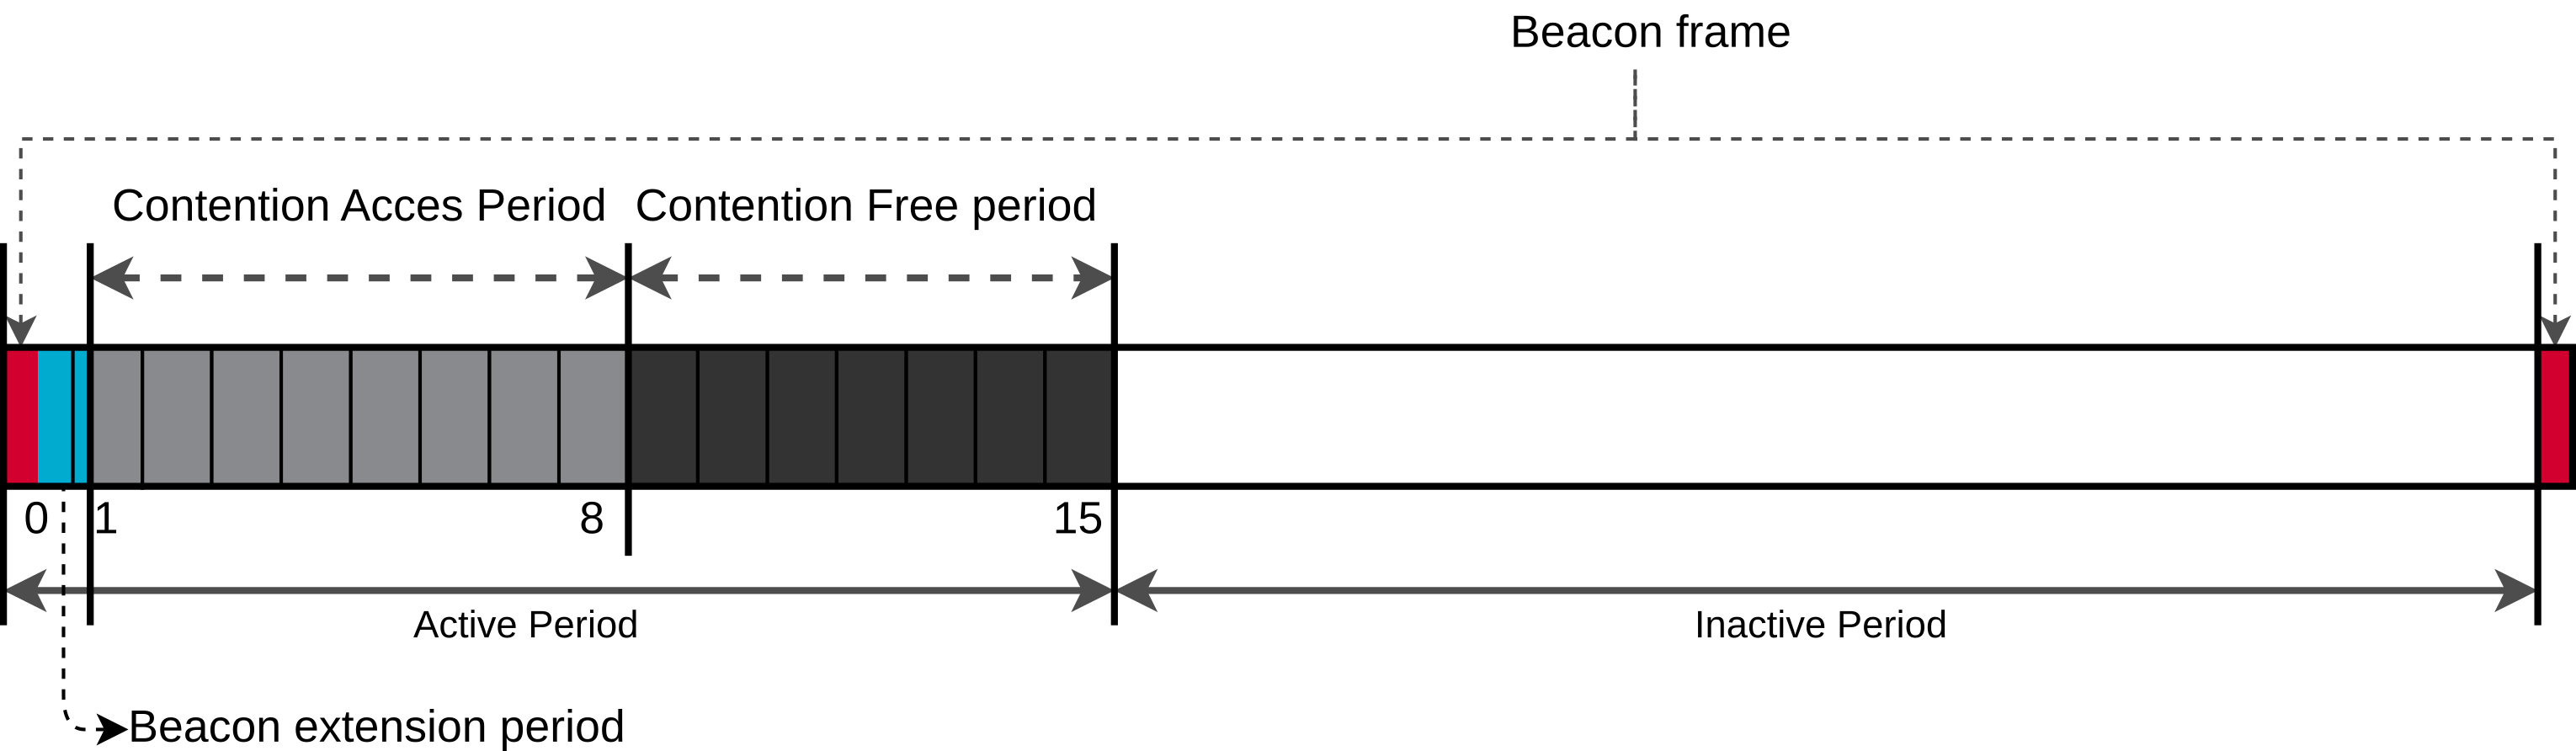
\includegraphics[scale=0.8]{res/pictures/superframe.png}
        }
        \caption{802.15.4 structure de la Superframe.}
        \label{fig:etat_art-802.15.4.superframe}
    \end{figure}

    Dans le mode Non-Beacon Enabled, il n'y a pas de synchronisation. l'accès au canal se fait par l'algorithme Unslotted CSMA-CA.


\subsection*{IEEE 802.15.4e}
    802.15.4 a un certains nombres de limitations. \cite{paper:802.15.4e-survey} met les limitations suivantes en évidence:
    \begin{itemize}
      \item Aucune garantie sur le délai maximal pour qu'un paquet puisse atteindre sa destination
        ne peut être fourni avec l'alorithme CSMA-CA.
      \item La fiabilité des communications est limitée par l'utilisation de l'algorithme slotted   CSMA-CA qui offre un taux de transmission faible.
      \item Aucune protection contre les interférences due à l'utilisation d'un seul canal et à     l'absence de mécanismes de sauts de fréquence (frequency hopping)
    \end{itemize}
    Ces limitations ont menées à la création de 802.14.4.e en 2012 qui redifinis les protocoles MAC du  standard.
    Ainsi, 5 modes de fonctionnement de la couche MAC sont introduis:
    \begin{enumerate}
      \item Time Slotted Channel Hopping (TSCH)
        %Cible les applications tel que l'automatisation de processus. Permet des communications    %multi-sauts et multi-canaux.
      \item Deterministic and Synchronous Multi-channel Extension (DSME)
        %Réalisé pour des applications industirelles et commercialesayant des contraintes de délai et
        %fiabilité. Permet des communications multi-sauts ainsi que la création de réseaux MESH.
      \item Low Latency Deterministic Network (LLDN)
        %Conçu pour les applications nécessitant une latence faible et les réseaux n'utilisant qu'un seul
        %canl pour des chemins d'un saut maximum.
      \item Asynchronous multi-channel adaptation (AMCA)
        %Cible les applications où de grands déploiments sont nécessaire comme le monitoring    %d'infrastructures.
      \item Radio Frequency Identification Blink (BLINK)
        %Conçu pour i'identification de personnes ou d'objets. Il permet aux noeuds de communiquer leur
        %ID aux autres noeuds sans avoir été préalablement associés.
    \end{enumerate}
    D'après \cite{paper:802.15.4e-survey}, le standart ne définit que brièvement AMCA et BLINK.
    LLDN est destiné aux réseaux à un seul saut et utilisant un seul canal. Il n'est donc pas pertinent pour ce projet. DSME utilise le concept de multi-superframe semblable aux superframe de IEEE 802.15.4 mise à part la CFP qui divie chacun des 7 slots en plusieurs fréquences.


\subsection{TSCH (Time Slotted Channel Hopping)}\label{subsec:etat_art-802.15.4.tsch}

Ce mode de fonctionnement de la couche MAC, comme son nom l'indique, supporte à la fois les sauts en fréquence et des communications divisées en temps. Ces mécanismes réduisent efficacement les effets des interférences et les collisions ce qui améliore la fiabilité du réseau.

\subsubsection*{Slotframe}
Dans ce mode, le concept de superframe de 802.15.4 est remplacé par le concept de slotframe.
Une slotframe est un intervalle de temps qui divisé en timeslots. Chaque timeslot permet à un noeud d'envoyer une trame et d'éventuellement recevoir son acquitement (ack).
Chaque timeslot possède un identifiant appellé \textit{Absolute Slot Number} (ASN)
et un identifiant au sein de la slotframe appelé \textit{Time Slot Number} (TSN).

TSCH permet l'utilisation de timeslots partagés et dédiés. Dans les timeslots partagés plusieurs noeuds peuvent communiquer. Dans ce cas, CSMA/CA est utilisé. Pour les timeslots dédiés, seul deux noeuds peuvent communiquer. La figure~\ref{fig:state-slotframe} illustre une slotframe composée de trois timeslots.
Dans cet exemple, on considère 3 noeuds: N, T et U. Chaque timeslot permet une communication entre deux noeud.
Par exemple le timeslot ayant comme TSN 0, permet à N de transmettre vers T.

\begin{figure}[H]
  \centering
  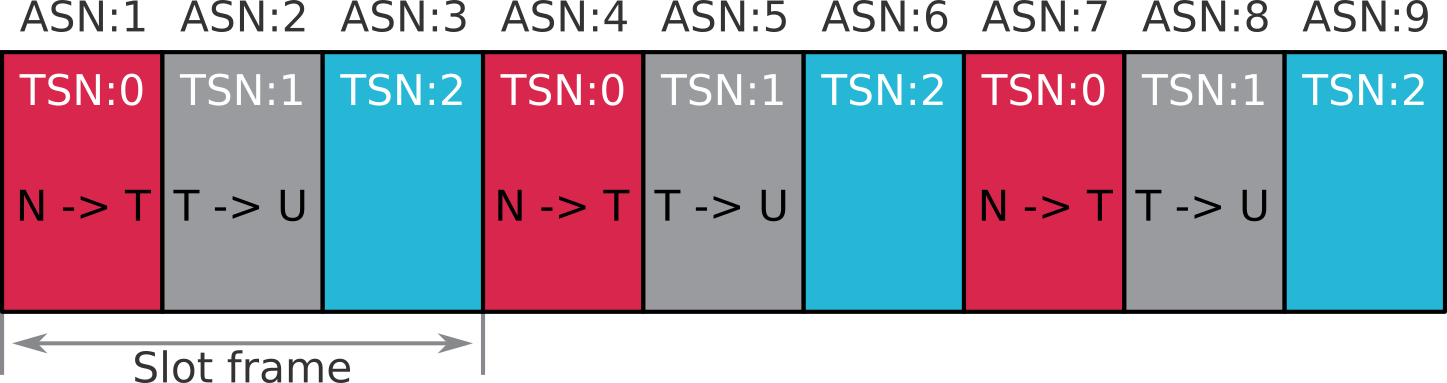
\includegraphics[scale=0.7]{res/pictures/sloframe.png}
  \caption{Slotframe.}
  \label{fig:state-slotframe}
\end{figure}

\subsubsection*{Channel Hopping}

TSCH peut utiliser 16 canaux différents numérotés de 0 à 15. Un lien entre deux noeuds dans TSCH est alors défini par la paire (timeslot, canal). Ainsi, chaque slot frame est divisiée par le nombre de canaux utilisé dans le réseau (Fig.~\ref{fig:state-tsch}). figure~\ref*{fig:state-slotframe}  Soit f la fréquence utilisée pour la communication entre deux noeuds:

\[
    f = F[(ASN + channel Offset)\% N_{channels}]
\]

où $N_{channels}$ est le nombre de canaux utilisés pour le réseau. F peut être vue comme une table qui contient une séquence de canaux.

\begin{figure}[H]
    \centering
    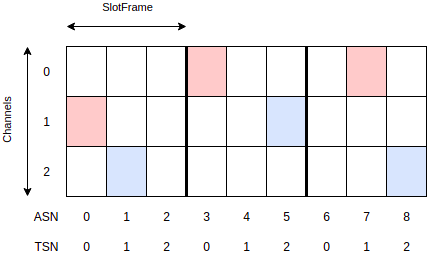
\includegraphics[scale=0.5]{res/pictures/tsch.drawio.png}
    \caption{Time Slotted Channel Hopping.}
    \label{fig:state-tsch}
\end{figure}


%\subsubsection*{Formation du PAN}

%\subsubsection*{Synchronisation en temps}
\newpage
\section{RPL}\label{sec:state-rpl}
\renewcommand{\rightmark}{RPL}
%TODO tour des protocoles de routages ??

Routing Protocol for Low-Power and Lossy Networks (RPL) est un protocole de routage IPv6 destiné aux réseaux dont les noeuds sont contraints en énergie et dont les liens entre ces noeuds sont soumis à des pertes importantes de paquets (Low-power and Lossy Networks (LLNs)).
Ce protocole à vecteur de distance est un protocole proactif, c'est à dire que les routes sont établies avant qu'elles ne soient nécessaires.

RPL sépare le traitement et la transmission des paquets de l'optimisation de l'objectif de routage. Cela permet de l'adapter à un large éventail d'applications des LLNs.

\subsection*{Topologie}
%TODO exemple de topologie + collect application noeuds-> racine
La topologie utilisée par RPL et le DODAG (Destination Oriented Dag). Un DODAG est un graphe dirigé acyclique (DAG) ayant une seule racine.
\begin{figure}[H]
    \centering
    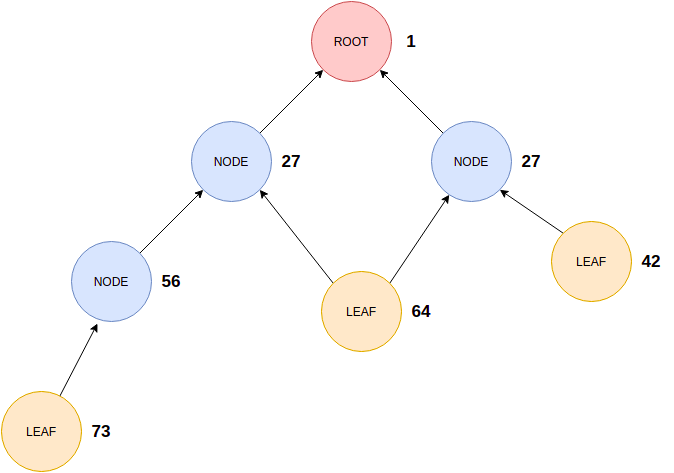
\includegraphics[scale=0.45]{res/dodag.drawio.png}
    \caption{DODAG.}
    \label{fig:state-dodag}
\end{figure}


\subsection*{Fonctions objectif}
%TODO expliquer brievement MRHOF et 0F0 (celles implémentées dans contiki)
Une fonction objectif (OF) défini comment plusieurs métriques sont utilisées pour calculer le rang d'un noeud. Le rang d'un noeud détermine sa position dans le DODAG par rapport aux autres noeuds.
Le rang augmente stictement dans le sens descendant et diminue strictement dans le sens montant. Ainsi, $rang(n)>rang(parent(n))$. La figure~\ref{fig:state-dodag} illustre un DODAG avec des valeurs de rang fictives attribuées aux noeuds. Sur cet exemple, la racine du DODAG a comme range, la valeur par défaut \textsc{root\_rank} définie dans le RFC.

Cette section décris brièvement deux fonctions objectif implémentées dans Contiki: OF0 et MRHOF.
\begin{itemize}
    \item \subsubsection*{OF0}%rfc6552
            Objective Function Zero est une fonction dont l'objectif est de choisir un parent qui permettra à un noeud d'avoir la racine du DODAG le plus proche possible. Le rang d'un noeud $R(N)$ est calculé comme suit:
                \[ranck\_increase = (Rf * Sp + Sr) * MinHopRankIncrease\]
                \[R(N) = R(P) + ranck\_increase\]
                où
                \begin{itemize}
                    \item[$\bullet$] $Rf$ est le $rank\_factor$ et $Sr \leq stretch\_of\_rank$ avec $rank\_factor$ et $stretch\_of\_rank$ deux paramètres de la fonction
                    \item[$\bullet$] $Sp$ est le $step_of_rank$ qui est une valeur basée sur les propriétés du lien
                    \item[$\bullet$] $MinHopRankIncrease$ est une constante
                    \item[$\bullet$] $R(p)$ est le rang d'un parent p
                \end{itemize}
                
    \item \subsubsection*{MRHOF}%rfc6719
            Minimum Rank with Hysteresis Objective Function est une fonction dont l'objectif est de 
\end{itemize}




\subsection*{Types de messages}
%TODO décrire le format des différents messages

\subsection*{Construction du réseau}
%TODO décrire les étapes de construction d'un réseau

\subsection*{Modes de fonctionnements}
%TODO parler des différents modes de fonctionnement: Storing mode/non-storing mode

\subsection*{Discussion}
%TODO RPL good parce que fait pour LLN (intro article eval RPL) et implémenté dans Contiki mais améliorations pour l'exterieur et grands réseaux (conclusion article eval RPL)
%%bib:
%@INPROCEEDINGS{5464820,
%  author={Tripathi, J. and de Oliveira, J. C. and Vasseur, J. P.},
%  booktitle={2010 44th Annual Conference on Information Sciences and Systems (CISS)}, 
%  title={A performance evaluation study of RPL: Routing Protocol for Low power and Lossy Networks}, 
%  year={2010},
%  volume={},
%  number={},
%  pages={1-6},
%  doi={10.1109/CISS.2010.5464820}}
\section{RTOS}

Un RTOS (Real Time Operating System) est un sytème d'exploitation temps réels principalement destiné aux systèmes embarqués.

Etant donné que ce projet utilise le protocole 802.15.4 ainsi que TSCH, le RTOS choisis doit les prendre en charge ainsi qu'un ou plusieurs algorithme d'ordonnancement de TSCH

Il est également préférable, que le RTOS choisis, supporte déjà la plateforme utilisée. Une implémentation de la LoRa n'est pas nécessaire car les communications Lora sont réalisées via le RN2483 qui est controlé par UART.

Pour effectuer ce choix, les RTOS suivants ont été comparés: Contiki OS, FreeRTOS, RIOT OS et Zephyr.

\subsection*{Contiki OS}
    Le développement publique de Contiki a débuté en octobre 2012\footnote{Date de création du repository Github.} Dans un premier repository: contiki~\cite{contiki-repo:old}. Un nouveau développement a démarré en mai 2017 sous le nom de Contiki-NG~\cite{contiki-repo:ng}. C'est donc ce dernier qui est utilisé pour la comparaison est qui est dénommé par la suite Contiki.

    Cet OS open-source et multi-plateforme implémente toute une série de protocoles de communications basse énergie tels que IEEE 802.15.4, 6TiSCH, IPv6/6LoWPAN et RPL. En plus de 6TiSCH, un ordonnanceur TSCH, Orchestra, est implémenté.
    TODO udp/tcp

    Contiki est également compatible avec le Zolertia RE-Mote. Il est accompagné de Cooja, un simulateur réseau qui permet de simuler les communications entre plusieurs noeuds utilisant Contiki.

\subsection*{FreeRTOS}
    D'après le site officiel de FreeRTOS~\cite{freertos}, ce RTOS est développé depuis 15 ans.
    TODO compatible avec zolertia ?

    \subsection*{RIOT OS}
    Le développement publique de RIOT a débuté en décembre 2012\footnotemark[1].
    
    D'après le site officiel, cet OS supporte 229 carte de développement et 64 CPU dont le Zolertia RE-Mote. 

    La pile réseau de RIOT comporte les protocoles notemment 6LoWPAN, IPv6, RPL, LoRaWan, 802.15.4.

\subsection*{Zephyr}
    TODO

Le table~\ref{tb:state-rtos-choice} résume la comparaison de ces RTOS.

Le RTOS choisi est Contiki OS. Il a été choisi pour sa maturié, la prise en charge du Zolertia RE-Mote et sa pile réseau complète.


%https://github.com/Lora-net/LoRaMac-node/blob/ba17382bd5109513937afad07f068a781a503ef6/src/radio/radio.h
\begin{table}[H]
    \begin{adjustbox}{width=\textwidth}
        \begin{tabular}{c||c|c|c|c|c|c|c}
            RTOS & 802.15.4 & ord. TSCH & LoRa & IPv6 & routage IP & comp. \\ \hline

            \textbf{Contiki OS} & $\surd$  & 6Tisch, Orchestra & Projet KRATOS & $\surd$ & RPL        & $\surd$ \\ \hline

            FreeRTOS            & $\times$ & $\times$          & $\surd$       & $\surd$ & $\times$   &    $\times$     \\ \hline

            RIOT OS             & $\surd$  & $\times$          & $\surd$       & $\surd$ & RPL        &    $\surd$     \\ \hline

            Zephyr              & $\surd$  & $\times$          & $\surd$       & $\surd$ & Thread     &    $\times$     \\
        \end{tabular}
    \end{adjustbox}
    \caption{Comparatif de différents RTOS.}
    \label{tb:state-rtos-choice}
\end{table}

\renewcommand{\leftmark}{ARCHITECTURE}
\chapter{Architecture}\label{chap:archi}

\section{Topologie}\label{sec:archi-topologie}
\renewcommand{\rightmark}{Topologie}

Cette section décrit et motive la topologie et les types de noeuds du réseau de capteurs hybride IEEE 802.15.4-LoRa. Cette topologie a été choisie pour correspondre au mieux au cas d'utilisation décrit dans l'introduction.\todo{REF INTRO + à savoir ...}

\subsection*{Types de noeuds}
    Le protocole élaboré pour ce réseau hybride définit 3 types de noeuds:
    \begin{itemize}
        \item[-] La \textbf{racine LoRa} est la passerelle entre le réseau et un réseau IP externe. Elle possède donc une interface LoRa et par exemple une interface Wi-Fi, Ethernet ou 3G/4G.
        \item[-] Les \textbf{racines RPL} sont les racines des réseaux RPL. Elles possèdent une interface LoRa pour communiquer avec la racine LoRa et une interface 802.15.4 pour communiquer avec les noeuds du réseau RPL.
        \item[-] Les \textbf{noeuds RPL} sont des noeuds des réseaux RPL.
    \end{itemize}

\subsection*{Topologie}
Comme l'illustre la figure~\ref{fig:archi-topologie} la topologie choisie est une topologie mixte.

On a d'abord un ensemble de réseaux RPL possèdant chacun un préfixe de sous-réseau IP attribué par la racine LoRa (par exemple $0x02$ ou $0x04$ sur la figure~\ref{fig:archi-topologie}), dans lesquels les communications se font par IEEE 802.15.4.
Comme RPL est utilisé, chaque réseau forme un DODAG.

Ensuite, chaque réseau RPL est connecté à la racine LoRa via sa racine RPL. Les liens entre les racines RPL et la racine LoRa forment une topologie en étoile.

%Ce choix de topologie offre plusieurs avantages: Le fait d'avoir un ensemble de réseaux RPL %implique qu'il n'y a pas qu'une seule racine RPL et donc pas qu'un seul point de défaillance; %L'administration du réseau est également simplifiée. En effet, un réseau RPL pourrait, par exemple, %correspondre à une parcelle de terrain.

Ce choix de topologie a comme avantage de simplifier l'administration du réseau. En effet, un réseau RPL pourrait, par exemple, correspondre à une parcelle de terrain. Comme cette topologie est composée d'un ensemble de réseau RPL, la défaillance d'une racine RPL pourrait impliquer la déconnexion d'un réseau RPL, contrairement à une topologie qui utilise un seul réseau RPL où la défaillance de la racine pourrait impliquer la déconnexion de l'ensemble des noeuds.

L'inconvéninent de cette topologie est que la racine LoRa constitue un seul point de défaillance. Une solution plus robuste qui a été envisagée, est un réseau maillé pour les communications LoRa. Cependant, une telle architecture est difficile à mettre en oeuvre car le protocole MAC a établir pour les liens LoRa est plus complexe et nécessite un protocole de routage.

\begin{figure}[H]
    \centering
    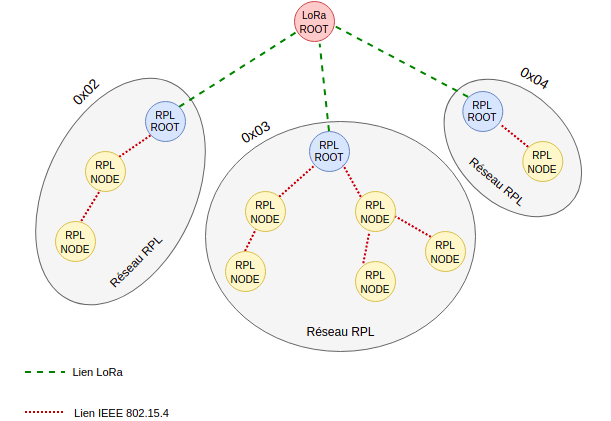
\includegraphics[scale=0.7]{res/pictures/loramac-topologie.drawio.png}
    \caption{Topologie du réseau hybride.}
    \label{fig:archi-topologie}
\end{figure}

%Ainsi, l'objectif de cette topologie est de transmettre les paquets IP à destination de la racine %LoRa.

L'essentiel du travail consite donc à définir et mettre en place un protocole MAC utilisant LoRa pour les communications entre les racines RPL et la racine LoRa ainsi que les mécanismes permettant de passer d'un réseau à un autre. Le routage est le transfert des paquets dans les réseaux RPL est quand à lui assuré par RPL et IPv6. Les sections suivantes décrivent le protocole MAC mis en place pour les communications LoRa.
\section{Format d'adresse}\label{sec:archi-adresses}
\renewcommand{\rightmark}{Format d'adresse}

Cette section décris les possibilités envisagées pour le choix du format des adresses utilisées pour les communications LoRa et motive le choix d'un format. Dans chaque hypothèse, un réseau RPL possède un préfixe IPv6.

\subsection*{Adresse IPv6}
    La première solution envisagée est d'utiliser les adresses IPv6 des noeuds.
    Une racine RPL (resp. racine LoRa) peut ainsi vérifier si un paquet est destiné à son réseau
    via le préfixe de l'adresse de destintation.
    Cette solution est la plus simple à mettre en oeuvre car elle ne nécéssite pas de table de routage ou de processus de conversion d'adresse. Néanmoins la taille des adresses IP est de 128 bits.

\subsection*{Préfixe et \textit{node-id}}
    Le \textit{node-id} est un identifiant sur 16 bits de noeud utilisé dans Contiki. Son calcul, basé sur les deux derniers octets de l'adresse mac du noeud (link-layer address) est le suivant:
    \[
        node\_id = link\_addr[s-1] + (link\_addr[size -2] << 8)
    \]
    où s est la taille de la link-layer address.\\

    Le format d'adresse utilisée serait alors un préfixe sur 8 bits et le \textit{node-id} sur 16 bits ce qui fait un total de 24 bits.

    L'avantage de cette solution est que la taille des adresses est nettement réduite. Néanmoins, un processus de conversion est nécessaire ainsi qu'une table de conversion d'un \textit{node-id} vers une adresse MAC pour chaque noeud RPL. En effet, le calcul du \textit{node-id} ne permet de reconstituer l'adresse MAC de 64 bits à partir de celui-ci.

\subsection*{Préfixe et adresse MAC}
    Pour résoudre le problème de la conversion \textit{node-id}$\leftrightarrow	$ adresse MAC, cette solution consiste à remplacer le \textit{node-id} par l'adresse MAC d'un noeud.

    Cette solution permet une conversion d'adresse simple et la taille des adresses est de 72 bits (64 bits de l'adresse MAC et 8 bits du préfixe).

\subsection*{Solution retenue}
    La solution retenue est l'utilisation du préfixe de 8 bits et du \textit{node-id} car c'est la solution qui offre les adresses les plus courtes. Pour éviter l'utilisation d'une table de conversion \textit{node-id}$\leftrightarrow$ adresse MAC, une meilleure solution que d'utiliser les adresses MAC des noeuds et de modifier les 6 premiers octets de cette dernière. Cela permet de reconstituer une adresse IPv6 simplement, mais cela réduits le nombre d'adresses possible
    Malgré tout, le nombre d'adresse possible reste largement suffisant pour ce projet.

    %todo schéma conversion, adresse de la racine 
\section{Trames LoRaMAC}\label{sec:archi-loramac-frame}
\renewcommand{\rightmark}{Trames LoRaMac}

    Le protocole MAC mis en place pour les communications LoRa utilise un seul format de trames illustré à la figure~\ref{fig:archi-frame}.
    \begin{figure}[H]
        \centering
        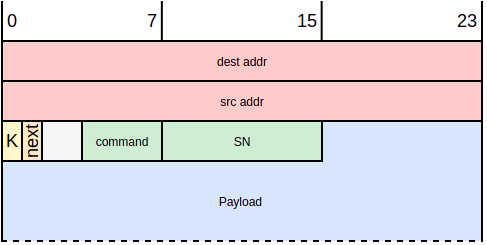
\includegraphics[scale=0.5]{res/pictures/loramac-frame.drawio.png}
        \caption{Format de trame LoRaMAC.}
        \label{fig:archi-frame}
    \end{figure}
    Les trames LoRaMAC sont composées des champs suivants:
    \begin{itemize}
        \item \textbf{dest\_addr}: l'adresse de destination (24 bits)
        \item \textbf{src\_addr}: l'adresse source (24 bits)
        \item \textbf{K}: un flag  qui indique si la trame nécessite un acquittement (1 bit)
        \item \textbf{next}: un flag qui indique si une autre trame suit (1 bit)
        \item \textbf{reserved}: 2 bits réservés pour évolution future
        \item \textbf{command}: la commande MAC (4 bits).\\
        Les 5 commandes disponibles ainsi que leurs valeurs sont reprises dans la table~\ref{tb:archi-loramac-command}. Il est possible d'ajouter 10 commandes supplémentaires pour des usages futurs.
        \item \textbf{SN}: le numéro de séquence de la trame (8 bits)
        \item \textbf{Payload}: la payload ayant une taille maximale de 247 octets. Cette limitation provient de la radio LoRa utilisée, le RN2483, qui limite les transmissions à 255 octets, valeur de laquelle est soustrait les 8 octets des champs précédents.
        \begin{table}[H]
            \centering
            \makebox[\textwidth]{%
            \begin{tabular}{|c|c|c|c|}
                \hline
                Valeur & Commande & description & payload\\ \hline
                0 & JOIN & requête pour rejoindre le réseau & $\times$ \\ \hline
                1 & JOIN\_RESPONSE & réponse à la commande JOIN & préfixe du sous réseau\\ \hline
                2 & DATA & transport de données & données\\ \hline
                3 & ACK & acquittement & $\times$\\ \hline
                4 & QUERY & demande de trafic descendant & $\times$\\ \hline
            \end{tabular}
            }
            \caption{Description des commandes LoRaMAC.}
            \label{tb:archi-loramac-command}
        \end{table}
    \end{itemize}

\section{LoRaMAC}\label{sec:archi-loramac:proto}
\renewcommand{\rightmark}{LoRaMac}

    Cette section décris le protocole MAC mis en place pour les communications LoRa. Ce protocole est donc utilisé pour les communications entre la racine LoRa et les racines RPL. Ces dernières étant contraintes en énergie, leur radio LoRa n'est pas tout le temps allumée. Le protocole prend donc en compte cette contrainte.

\subsection*{Etats d'une Racine RPL}
    Les racines RPL utilisent 4 états illustrés dans le diagramme d'état de la figure~\ref{fig:archi-state}. A l'initiation du réseau, une racine RPL se trouve dans l'état \textit{alone}. Elle demande ensuite son préfixe à la racine LoRa. Si la transmission échoue trop de fois, elle entre dans l'état \textit{sleep} dans lequel ses radios sont éteintes, jusqu'à ce que l'évènement \textit{wake up} soit déclenché pour retourner dans l'état \textit{alone}. Si la transmission est réussie, et donc que le préfixe est reçu, la racine RPL se trouve dans l'état \textit{ready}. Quand une racine RPL envoie une trame qui nécessite un acquittement, tant que celui-ci n'est pas reçu elle se trouvera dans l'état \textit{wait\_response}. Une fois l'acquittement reçu, elle retournera dans l'état \textit{ready}.
    
    Les trames qui doivent être envoyées le seront en fonction de l'état dans lequel se trouve une racine RPL. Dans l'état \textit{ready}, les trames de données peuvent être envoyées, mais ce n'est pas le cas dans les états \textit{alone} et \textit{wait\_response}. En effet, dans le premier état, la racine RPL ne peut pas envoyer de données car elle n'a pas encore rejoint le réseau et dans le second, elle attend une réponse.
    \begin{figure}[H]
        \centering
        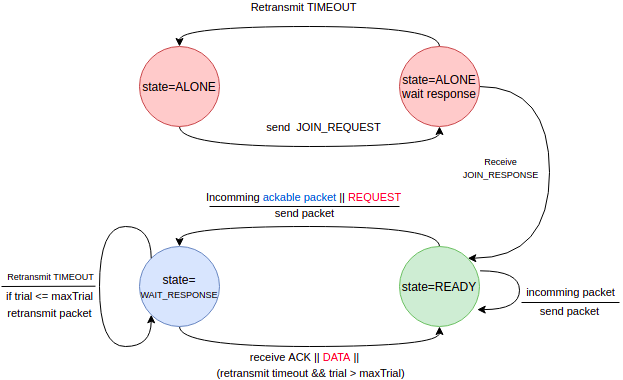
\includegraphics[scale=0.5]{res/pictures/loramac-state.drawio.png}
        \caption{Diagramme d'état des racines RPL.}
        \label{fig:archi-state}
    \end{figure}

\subsection*{Etats de la racine LoRa}
    Le diagramme d'état de la racine LoRa pour chaque racine RPL qui a rejoint le réseau est 
    illustré à la figure~\ref{fig:archi-state-lora}. Une fois que la racine RPL (enfant de la 
    racine LoRa) a rejoint le réseau, l'état est READY. Cela signifie que la racine LoRa est prête 
    à recevoir des données de cet enfant. Si elle reçoit une trame DATA, les données sont 
    transmises à la couche supérieure. Elle peut donc rester dans le même état. Elle reste aussi 
    dans l'état READY si elle reçoit une QUERY et qu'il n'y a aucune données disponible pour cet 
    enfant. En revanche, si des données sont disponibles, la racine LoRa entre dans l'état TRANSMIT 
    dans lequel elle va envoyer tous les paquets disponibles pour cet enfant. Une fois dans l'état 
    TRANSMIT la racine LoRa envoie un paquet et bascule dans l'état WAIT TIMER dans lequel elle 
    attend une possible demande de retransmission de son enfant. Si une retransmission est 
    demandée, le timer est réinitialisé. Une fois le timer expiré, elle retourne dans l'état 
    TRANSMIT. S'il n'y a plus de données pour cet enfant, elle retourne dans l'état READY.

    %Cela permet également d'éviter que l'état d'un autre enfant bascule dans READY ce qui mettrait la radio en mode écoute alors qu'elle essaye de transmettre des paquets pour cet enfant. Cela bloquerait donc les transmissions pour cet enfant.

    \begin{figure}[H]
        \centering
        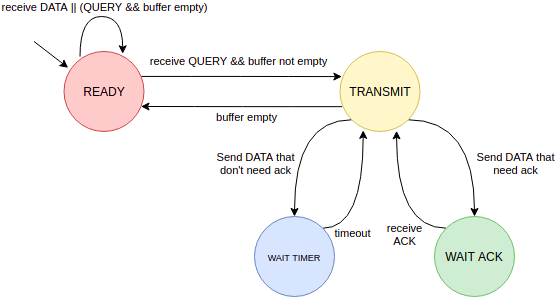
\includegraphics[scale=0.5]{res/pictures/loramac-loraroot-state.drawio.png}
        \caption{Diagramme d'état de la racine LoRa.}
        \label{fig:archi-state-lora}
    \end{figure}

\subsection*{Construction du réseau}%done
    A l'initialisation du réseau, une racine RPL doit envoyer une trame avec la commande JOIN. Une 
    fois reçue par la racine LoRa, celle-ci va répondre avec une trame JOIN\_RESPONSE qui fait 
    office d'acquittement de la trame JOIN et dont la payload est le préfixe du réseau de la racine 
    RPL qu'elle doit diffuser dans son réseau.

    Si la trame JOIN ou la trame JOIN\_RESPONSE ne sont pas reçues, la racine RPL retransmettra la 
    trame JOIN à l'expiration d'un timer \textit{retransmit\_timer} déclenché à l'envoi de la trame 
    JOIN. Cette retransmission se répète au maximum \textsc{max\_attempt} fois. Si ce seuil est 
    dépassé, la communication est considérée comme échouée. Dans ce cas, la racine attend $w$ 
    secondes avant de répéter le processus. $w$ est défini par l'équation~\ref{eq:archi-wait}, 
    dans laquelle, $r$ est le temps ajouté au $retransmit\_timeout$ qui est le temps après lequel 
    le timer \textit{retransmit\_timer} expire. $r$ est le modulo $retransmit\_timeout$ d'un nombre 
    $rand$ qui doit être choisi aléatoirement.
    \begin{equation}\label{eq:archi-wait}
        \begin{split}
            r = rand \% retransmit\_timeout \\
            w = (retransmit\_timeout + r) \% 60
        \end{split}
    \end{equation}
    
    Une fois le préfixe reçu, la racine RPL peut initialiser le réseau RPL et y diffuser le préfixe.

    Le diagramme de séquence de la figure~\ref{fig:proto-seq-join} illustre le processus de construction du réseau.
    \begin{figure}[H]
        \centering
        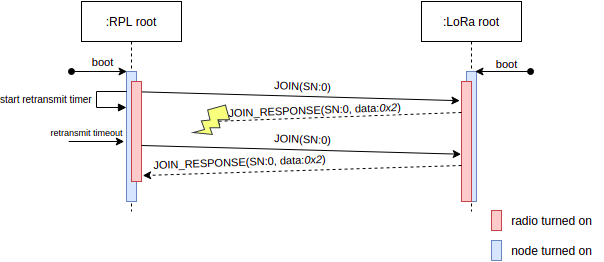
\includegraphics[scale=0.6]{res/pictures/loramac-sequence-JOIN.drawio.png}
        \caption{Diagramme de séquence de la construction du réseau.}
        \label{fig:proto-seq-join}
    \end{figure}

\subsection*{Communications montantes}%done
    Lorsqu'un paquet est destiné à une adresse IPv6 externe au réseau d'une racine RPL, il va remonter jusqu'à celle-ci, qui va ensuite l'envoyer à la racine LoRa.

    Si la trame envoyée à la racine LoRa nécessite un acquittement, la racine RPL n'enverra pas d'autres trames tant que l'acquittement n'a pas été reçu (état \textit{wait\_response}).
    A l'envoi de cette trame, le timer \textit{retransmit\_timer} est déclenché. S'il expire avant que l'acquittement ne soit reçu, la trame sera retransmise pour un maximum de 3 fois.
    Arpès 3 transmissions qui n'ont pas réussi, la racine RPL retourne dans l'état READY et le paquet est perdu.

    Si la trame envoyée à la racine LoRa ne nécessite pas d'acquittement, la réception de cette trame n'est pas garantie et la racine RPL peut directement transmettre les trames suivantes s'il y en a.

    Le diagramme de séquence de la figure~\ref{fig:proto-seq-upward} illustre le déroulement des communications montantes.
    \begin{figure}[H]
        \centering
        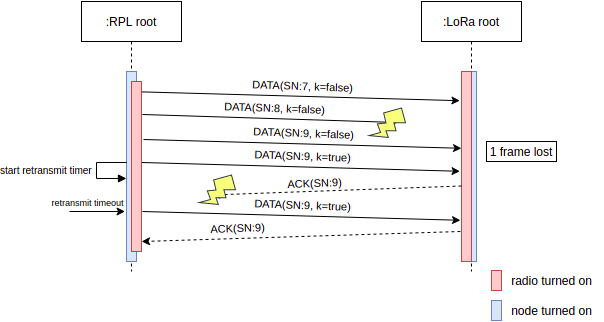
\includegraphics[scale=0.6]{res/pictures/loramac-sequence-UPWARD.drawio.png}
        \caption{Diagramme de séquence du trafique montant.}
        \label{fig:proto-seq-upward}
    \end{figure}    

\subsection*{Communications descendantes}%done
    La racine LoRa possède un buffer pour chaque réseau RPL dans lequel elle accumule les paquets destinés à ce réseau. Pour chaque racine RPL, lors de l'expiration, à intervalle régulier, du timer \textit{query\_timer}, une trame avec la commande QUERY est transmise à la racine LoRa.

    La réponse à cette trame doit être un acquittement, si la racine LoRa n'a pas de paquets pour le réseau de cette racine RPL, ou une trame avec la commande DATA si un ou plusieurs paquets sont disponibles.

    Si la racine LoRa possède plusieurs paquets à destination du même réseau RPL, la valeur du flag \textit{next} doit être à 1 pour toutes les trames envoyées à l'exception de la dernière.

    Comme pour les communications montantes, les retransmissions sont initiées par les racines RPL.
    Le timer \textit{retransmit\_timer} est activé lorsque la QUERY est envoyée ou lorsqu'une trame DATA avec le flag \textit{next} à 1 est reçue.

    Les acquittements ne sont pas nécessaires pour les communications descendantes, car, si la racine LoRa envoie une trame, cela signifie qu'une racine RPL attend cette trame. Si elle n'est pas reçue, la racine RPL demandera une retransmission via l'envoi de la dernière trame envoyée, c'est à dire la trame avec la commande QUERY.

    Après 3 retransmissions, le paquet est perdu et le prochain sera transmis lors de la réception d'une QUERY.

    Le diagramme de séquence de la figure~\ref{fig:proto-seq-downward} illustre le déroulement des communications descendantes.
    \begin{figure}[H]
        \centering
        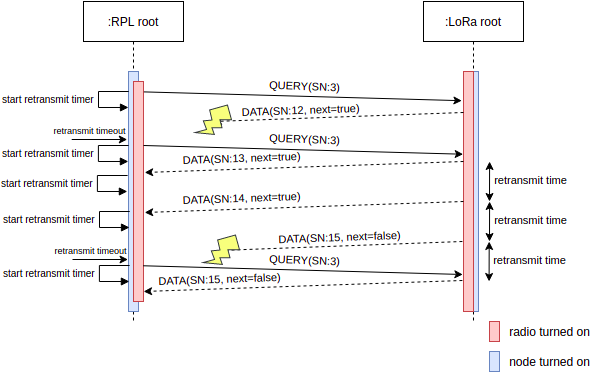
\includegraphics[scale=0.6]{res/pictures/loramac-sequence-DOWNWARD.drawio.png}
        \caption{Diagramme de séquence du trafic descendant.}
        \label{fig:proto-seq-downward}
    \end{figure}


    %Si une trame nécessite un acquittement et que l'acquittement n'est pas reçu, la racine LoRa %n'envoie pas le paquet suivant. Dans ce cas deux situations sont possibles:
    %\begin{itemize}
    %    \item La trame avait le flag \textit{next} à 1:\\
    %        La racine RPL s'attend à une autre trame. L'acquittement va donc être retransmis à %l'expiration du \textit{retransmit\_timer} avec un maximum 3 retransmissions.
    %    \item La trame avait le flag \textit{next} à 0:\\
    %        La racine LoRa retransmettra le paquet concerné lors de la réception d'une QUERY.
    %\end{itemize}

\subsection*{Gestion des numéros de séquence}
    Les racines RPL et la racine LoRa possèdent deux compteurs: \textit{expected\_sn} et \textit{next\_sn}.

    La valeur du compteur \textit{expected\_sn} est le numéro de séquence attendu de la prochaine trame reçue. Ce compteur permet de savoir si une trame a été perdue. Sa valeur est le numéro de séquence de la dernière trame reçue incrémenté de 1.

    La valeur du compteur \textit{next\_sn} est le numéro de séquence de la prochaine trame. Il est incrémenté de 1 lorsqu'une trame a été envoyée.

    Les deux compteurs sont initialisés à zéro.

%\subsubsection*{Exemple de communications}
%    Les figures~\ref{fig:archi-sequence1} et~\ref{fig:archi-sequence2} ci-dessous, illustrent le 
%    protocole LoRaMAC qui vient d'être décrit dans cette section. La première illustre les échanges 
%    de messages sans retransmissions et la deuxième avec retransmissions. Les détails des timers ne 
%    sont pas présents sur ces figures pour plus de clarté.
%    \begin{figure}[H]
%        \centering
%        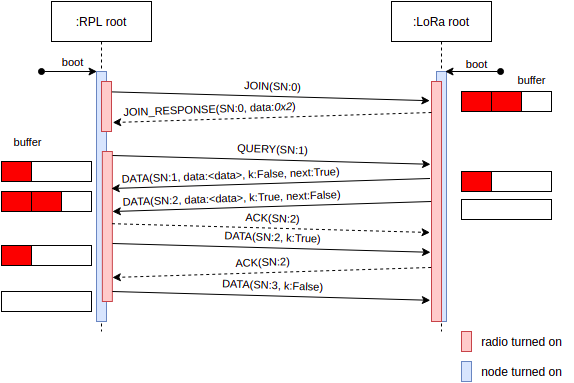
\includegraphics[scale=0.6]{res/pictures/loramac-sequence1.drawio.png}
%        \caption{Diagramme de séquence LoRaMAC.}
%        \label{fig:archi-sequence1}
%    \end{figure}
%    \begin{figure}[H]
%        \centering
%        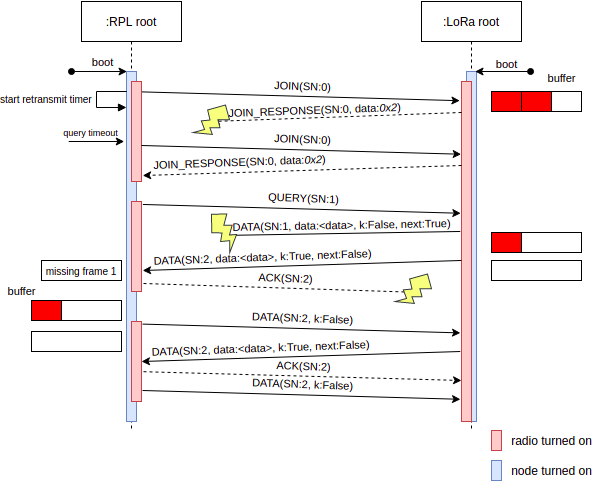
\includegraphics[scale=0.6]{res/pictures/loramac-sequence2.drawio.png}
%        \caption{Diagramme de séquence LoRaMAC avec retransmissions.}
%        \label{fig:archi-sequence2}
%    \end{figure}

%\subsection{Evitement de collision}
%    L'envoi des trames est réalisé avec l'algorithme CSMA/CA pour les racines RPL. 
%    Avant l'envoi, ces noeuds écoute le canal. Si le canal est occupé, le noeud va resonder le
%    canal après un temps aléatoire. Ce processus se répète 3 fois. Après ces trois fois, si le
%    canal est toujours occupé, la trame ne sera pas envoyée. A chaque sondage du canal, l'interval
%    dans lequel le temps aléatoire est choisi est agrandit. Si le canal n'est pas occupé, la trame
%    est envoyée.

%\section{Plateformes de développement}\label{sec:etat_art-802.15.4}
\renewcommand{\rightmark}{Plateformes de développement}
\subsection*{Zolertia RE-Mote}
Pour ce mémoire, la plateforme Zolertia RE-Mote revision B(Fig.~\ref{fig:state-zolertia}) est utilisée.

Cette plateforme, basée sur un system on chip (SoC) CC2538 ARM Cortex-M3, a été conçue par des universités et des industriels dans le but de permettre aux chercheurs et makers de développer des applications IoT et des objets connectés.

Le Zolertia RE-Mote a été choisi car elle est équipée de deux radios compatibles IEEE 802.15.4,
permet une consommation électrique faible et possède de nombreux pins de connexion qui peuvent être utilisés pour y connecter des capteurs, actuateurs, radios, etc.

Le prix du consturcteur pour cette plateforme est de 93,95€~\cite{zolertia-remote:shop}.

\begin{figure}[H]
    \centering
    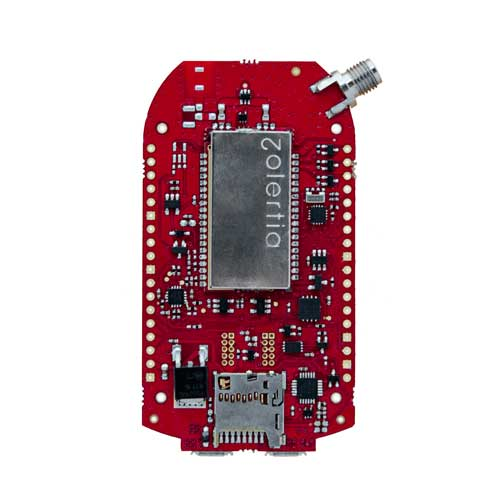
\includegraphics[scale=0.3]{res/pictures/remote-zolertia.jpg}
    \caption{Zolertia RE-Mote révision B~\cite{zolertia-remote:shop}.}
    \label{fig:state-zolertia}
\end{figure}

La table~\ref{tb:state-spec} reprend les principales spécifications du Zolertia RE-Mote rev.b et sa table ... la consommation électique.%TODO datasheet ???

\begin{table}[H]
    \centering
    \begin{tabular}{|c|c|}
        \hline
        \rowcolor{lightgray}
        Element            & Spécification\\
        \hline
        Radio              & Deux radios IEEE 802.15.4 à 2.4 GHz et 863-950 MHz\\
        \hline
        CPU                & ARM\textsuperscript{\tiny\textregistered} Cortex\textsuperscript{\tiny\textregistered} -M3 jusqu'à 32 MHz\\
        \hline
        RAM                & 32 KB (16 KB pour tous les Power Modes)\\
        \hline
        Flash programmable & 512KB\\
        \hline
        I/O                & RGB led, boutton user et reset, USB 2.0 à 12Mbps, Real-Time Clock\\
        \hline
    \end{tabular}
    \caption{Spécifications du Zolertia RE-Mote rev.b~\cite{zolertia-remote:datasheet}.}
    \label{tb:state-spec} reprend la consommation de courant du RN2483 
\end{table}

\subsection*{RN2483}
    Le RN2483 (Fig.~\ref{fig:state-rn2483}) est un modem LoRa compatible LoRaWAN$^{TM}$ basse énergie.
    La communication avec ce modem ce fait par des commandes ASCII envoyée via une interface UART. Il prend en charge les modulations FSK, GFSK et LoRa. Il possède également 14 GPIOs ??pour le contrôle et le status, partagés avec 14 inputs analogiques.??%TODO
    Ses fréquences opérationnelles sont situées dans les bandes de fréquences 433 MHz et 868 MHz. D'après la datasheet, 
    sa portée maximale est de 15km en agglomération et 5km en zone urbaine. Comme l'illustre la figure.~\ref{fig:state-rn2483}, pour ce mémoire, le RN2483 a été monté sur un carte d'interface réalisée par B.Quoitin qui comporte deux leds, une petite antenne ainsi que les connecteurs permettant d'utiliser des câbles de prototypages.

    \begin{figure}[H]%TODO changer figure
        \centering
        
\includegraphics[scale=0.3]{res/pictures/rn2483.png}
        \caption{RN2483~\cite{rn2483:shop}.}
        \label{fig:state-rn2483}
    \end{figure}

    La figure \ref{fig:state-rn2484-block} reprend le schéma-bloc du RN2483. Il contient notemment l'interface UART, les antennes 433 MHz et 868Mhz ainsi que les GPIOs et la stack LoRaWan.
    \begin{figure}[H]
        \centering
        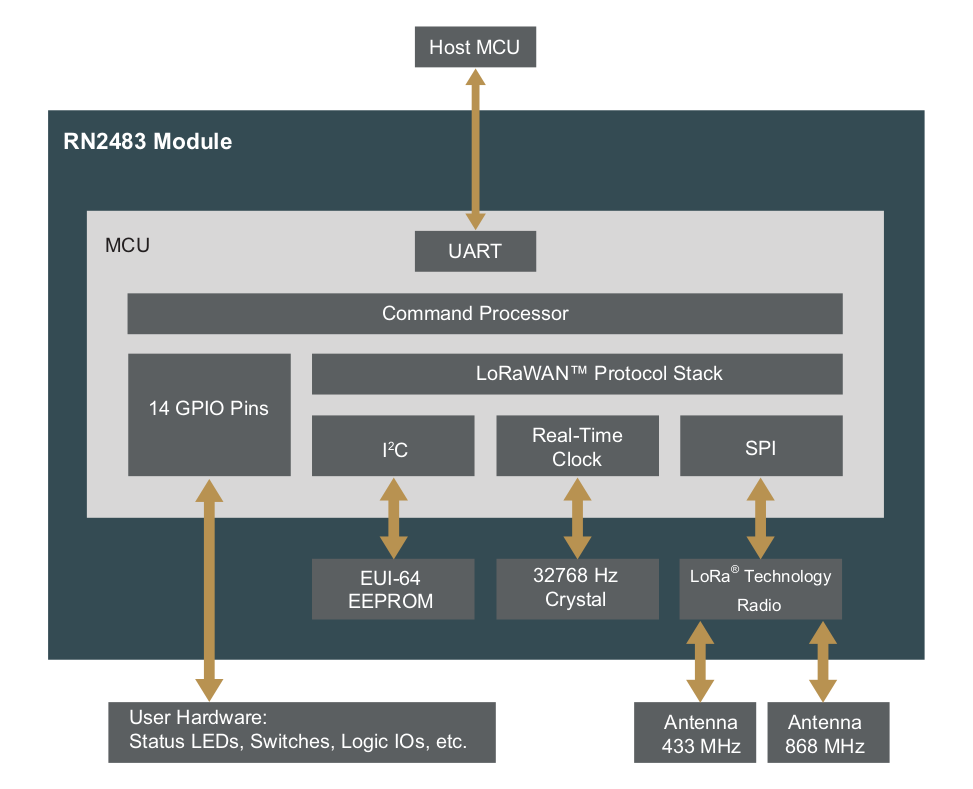
\includegraphics[scale=0.4]{res/pictures/rn2483-block-diagram.png}
        \caption{Schéma-bloc du RN2483~\cite{rn2483:datasheet}.}
        \label{fig:state-rn2484-block}
    \end{figure}
    La table~\ref{tb:state-rn2483-consumption} reprend la consommation électrique du RN2483 en fonction de son mode de fonctionnement.
    \begin{table}[H]
        \centering
        \begin{tabular}{| *{4}{c|} }
            \hline
            Mode & \multicolumn{3}{c|}{\multirow{1}{*}{Courant (mA)}}\\ \cline{2-4}
             & VDD = 2.1V & VDD = 3.3V  & VDD = 3.6V \\ \hhline{|=|=|=|=|}
            Idle & 1.7 & 2.8 & 3.1 \\ \hline
            Transmit & 28.6 & 38.9 & 44.5 \\ \hline
            Sleep & 0.0015 & 0.0016 & 0.0016 \\ \hline
            Receive & 12.96 & 14.22 & 14.69 \\ \hline
        \end{tabular}
        \caption{Consommation de courant (à 25 °C) \cite{rn2483:datasheet}.}
        \label{tb:state-rn2483-consumption}
    \end{table}

\subsection*{Raspberry Pi}

Le Raspberri Pi est un ordinateur monocarte. Le modèle utilisé pour ce projet est un Raspberry Pi 3 modèle B+ (Fig.~\ref{fig:state-raspberrypi}). La table \ref{tb:state-raspberrypi-spec} reprend les principales caractéristiques de ce modèle.

\begin{figure}[H]
    \centering
    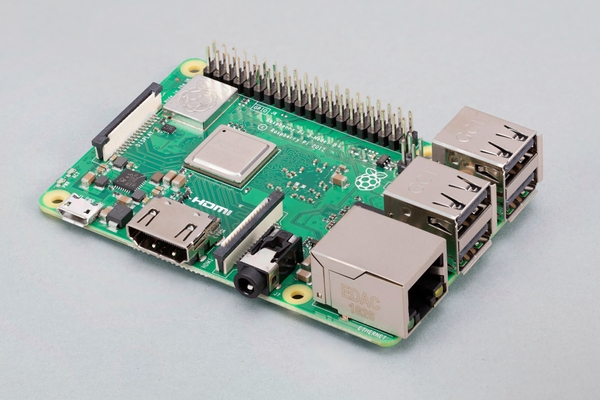
\includegraphics[scale=0.4]{res/pictures/raspberrypi3b+.png}
    \caption{Raspberry Pi 3B+~\cite{raspberry:shop}.}
    \label{fig:state-raspberrypi}
\end{figure}

\begin{table}[H]
    \centering
    \begin{tabular}{|c|p{0.75\textwidth}|}
        \hline
        \rowcolor{lightgray}
        Element            & Spécification\\
        CPU & Broadcom BCM2837B0, Cortex-A53 64-bit SoC à 1.4GHz\\ \hline
        Mémoire & 1GB LPDDR2 SDRAM \\ \hline
        Connectivité & 
        \begin{itemize}
            \item IEEE 802.11.b/g/n/ac, Bluetooth 4.2, BLE
            \item Gigabit Ethernet over USB 2.0
            \item 4 × USB 2.0 ports
        \end{itemize}\\ \hline
        Alimentation & 5V/2.5A DC\\ \hline
    \end{tabular}
    \caption{Spécifications du Raspberry Pi 3B+ \cite{raspberry:shop}.}
    \label{tb:state-raspberrypi-spec}
\end{table}

%\section{RTOS}

Un RTOS (Real Time Operating System) est un sytème d'exploitation temps réels principalement destiné aux systèmes embarqués.

Etant donné que ce projet utilise le protocole 802.15.4 ainsi que TSCH, le RTOS choisis doit les prendre en charge ainsi qu'un ou plusieurs algorithme d'ordonnancement de TSCH

Il est également préférable, que le RTOS choisis, supporte déjà la plateforme utilisée. Une implémentation de la LoRa n'est pas nécessaire car les communications Lora sont réalisées via le RN2483 qui est controlé par UART.

Pour effectuer ce choix, les RTOS suivants ont été comparés: Contiki OS, FreeRTOS, RIOT OS et Zephyr.

\subsection*{Contiki OS}
    Le développement publique de Contiki a débuté en octobre 2012\footnote{Date de création du repository Github.} Dans un premier repository: contiki~\cite{contiki-repo:old}. Un nouveau développement a démarré en mai 2017 sous le nom de Contiki-NG~\cite{contiki-repo:ng}. C'est donc ce dernier qui est utilisé pour la comparaison est qui est dénommé par la suite Contiki.

    Cet OS open-source et multi-plateforme implémente toute une série de protocoles de communications basse énergie tels que IEEE 802.15.4, 6TiSCH, IPv6/6LoWPAN et RPL. En plus de 6TiSCH, un ordonnanceur TSCH, Orchestra, est implémenté.
    TODO udp/tcp

    Contiki est également compatible avec le Zolertia RE-Mote. Il est accompagné de Cooja, un simulateur réseau qui permet de simuler les communications entre plusieurs noeuds utilisant Contiki.

\subsection*{FreeRTOS}
    D'après le site officiel de FreeRTOS~\cite{freertos}, ce RTOS est développé depuis 15 ans.
    TODO compatible avec zolertia ?

    \subsection*{RIOT OS}
    Le développement publique de RIOT a débuté en décembre 2012\footnotemark[1].
    
    D'après le site officiel, cet OS supporte 229 carte de développement et 64 CPU dont le Zolertia RE-Mote. 

    La pile réseau de RIOT comporte les protocoles notemment 6LoWPAN, IPv6, RPL, LoRaWan, 802.15.4.

\subsection*{Zephyr}
    TODO

Le table~\ref{tb:state-rtos-choice} résume la comparaison de ces RTOS.

Le RTOS choisi est Contiki OS. Il a été choisi pour sa maturié, la prise en charge du Zolertia RE-Mote et sa pile réseau complète.


%https://github.com/Lora-net/LoRaMac-node/blob/ba17382bd5109513937afad07f068a781a503ef6/src/radio/radio.h
\begin{table}[H]
    \begin{adjustbox}{width=\textwidth}
        \begin{tabular}{c||c|c|c|c|c|c|c}
            RTOS & 802.15.4 & ord. TSCH & LoRa & IPv6 & routage IP & comp. \\ \hline

            \textbf{Contiki OS} & $\surd$  & 6Tisch, Orchestra & Projet KRATOS & $\surd$ & RPL        & $\surd$ \\ \hline

            FreeRTOS            & $\times$ & $\times$          & $\surd$       & $\surd$ & $\times$   &    $\times$     \\ \hline

            RIOT OS             & $\surd$  & $\times$          & $\surd$       & $\surd$ & RPL        &    $\surd$     \\ \hline

            Zephyr              & $\surd$  & $\times$          & $\surd$       & $\surd$ & Thread     &    $\times$     \\
        \end{tabular}
    \end{adjustbox}
    \caption{Comparatif de différents RTOS.}
    \label{tb:state-rtos-choice}
\end{table}
%\newpage
\section{RPL}\label{sec:state-rpl}
\renewcommand{\rightmark}{RPL}
%TODO tour des protocoles de routages ??

Routing Protocol for Low-Power and Lossy Networks (RPL) est un protocole de routage IPv6 destiné aux réseaux dont les noeuds sont contraints en énergie et dont les liens entre ces noeuds sont soumis à des pertes importantes de paquets (Low-power and Lossy Networks (LLNs)).
Ce protocole à vecteur de distance est un protocole proactif, c'est à dire que les routes sont établies avant qu'elles ne soient nécessaires.

RPL sépare le traitement et la transmission des paquets de l'optimisation de l'objectif de routage. Cela permet de l'adapter à un large éventail d'applications des LLNs.

\subsection*{Topologie}
%TODO exemple de topologie + collect application noeuds-> racine
La topologie utilisée par RPL et le DODAG (Destination Oriented Dag). Un DODAG est un graphe dirigé acyclique (DAG) ayant une seule racine.
\begin{figure}[H]
    \centering
    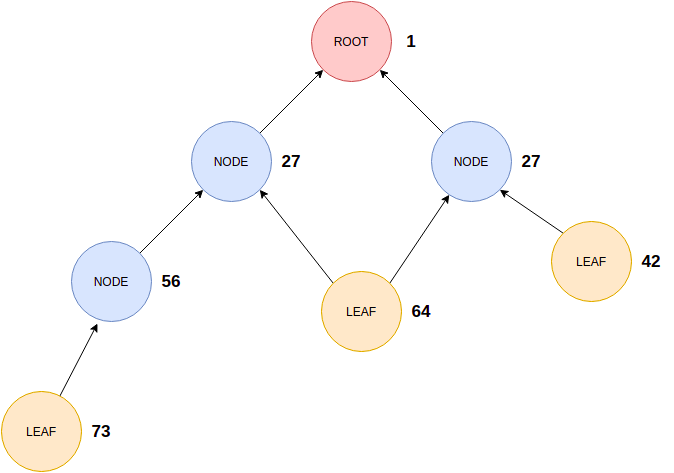
\includegraphics[scale=0.45]{res/dodag.drawio.png}
    \caption{DODAG.}
    \label{fig:state-dodag}
\end{figure}


\subsection*{Fonctions objectif}
%TODO expliquer brievement MRHOF et 0F0 (celles implémentées dans contiki)
Une fonction objectif (OF) défini comment plusieurs métriques sont utilisées pour calculer le rang d'un noeud. Le rang d'un noeud détermine sa position dans le DODAG par rapport aux autres noeuds.
Le rang augmente stictement dans le sens descendant et diminue strictement dans le sens montant. Ainsi, $rang(n)>rang(parent(n))$. La figure~\ref{fig:state-dodag} illustre un DODAG avec des valeurs de rang fictives attribuées aux noeuds. Sur cet exemple, la racine du DODAG a comme range, la valeur par défaut \textsc{root\_rank} définie dans le RFC.

Cette section décris brièvement deux fonctions objectif implémentées dans Contiki: OF0 et MRHOF.
\begin{itemize}
    \item \subsubsection*{OF0}%rfc6552
            Objective Function Zero est une fonction dont l'objectif est de choisir un parent qui permettra à un noeud d'avoir la racine du DODAG le plus proche possible. Le rang d'un noeud $R(N)$ est calculé comme suit:
                \[ranck\_increase = (Rf * Sp + Sr) * MinHopRankIncrease\]
                \[R(N) = R(P) + ranck\_increase\]
                où
                \begin{itemize}
                    \item[$\bullet$] $Rf$ est le $rank\_factor$ et $Sr \leq stretch\_of\_rank$ avec $rank\_factor$ et $stretch\_of\_rank$ deux paramètres de la fonction
                    \item[$\bullet$] $Sp$ est le $step_of_rank$ qui est une valeur basée sur les propriétés du lien
                    \item[$\bullet$] $MinHopRankIncrease$ est une constante
                    \item[$\bullet$] $R(p)$ est le rang d'un parent p
                \end{itemize}
                
    \item \subsubsection*{MRHOF}%rfc6719
            Minimum Rank with Hysteresis Objective Function est une fonction dont l'objectif est de 
\end{itemize}




\subsection*{Types de messages}
%TODO décrire le format des différents messages

\subsection*{Construction du réseau}
%TODO décrire les étapes de construction d'un réseau

\subsection*{Modes de fonctionnements}
%TODO parler des différents modes de fonctionnement: Storing mode/non-storing mode

\subsection*{Discussion}
%TODO RPL good parce que fait pour LLN (intro article eval RPL) et implémenté dans Contiki mais améliorations pour l'exterieur et grands réseaux (conclusion article eval RPL)
%%bib:
%@INPROCEEDINGS{5464820,
%  author={Tripathi, J. and de Oliveira, J. C. and Vasseur, J. P.},
%  booktitle={2010 44th Annual Conference on Information Sciences and Systems (CISS)}, 
%  title={A performance evaluation study of RPL: Routing Protocol for Low power and Lossy Networks}, 
%  year={2010},
%  volume={},
%  number={},
%  pages={1-6},
%  doi={10.1109/CISS.2010.5464820}}
%\section{IEEE 802.15.4e}\label{sec:etat_art-802.15.4}
\renewcommand{\rightmark}{IEEE 802.15.4e}
    802.15.4 est un protocole définis par IEEE en 2003. Il est destiné aux communications à débit faibles réalsisées par des dispositifs ayant une alimentation en énergie limitée.
    Ce protocole qui est un standart pour les réseaux PANs (Personak Area Networks) couvre la couche physique et MAC du modèle OSI. En 2012, IEEE 802.15.4e a été défini pour palier à certains problèmes de IEEE 802.15.4.

\subsection*{IEEE 802.15.4}
    \subsubsection*{Types de noeuds et topologie}
    Cette norme défini deux types de noeuds: les Full Function Devices (FFD) qui peuvent être des coordinateurs de PAN, de simple coordinateurs ou de simple noeuds et les Reduced Function Device (RFD) qui utilisent une implémentation réduite du protocole et ne peuvent être que de simples noeuds.

    Ces noeuds peuvent former des réseaux suivantes plusieurs topologies
    comme la topologie en étoile pour laquelle plusieurs RFD sont connectés à un FFD qui
    joue le rôle de coordinateur ou encore la topologie peer-to-peer pour laquelle les FFD sont connectés les uns aux autres.

    \subsubsection*{Modes d'accès}
    802.15.4 défini deux modes d'accès: Beacon Enabled mode et Non-Beacon Enabled mode.
    Dans le premier, le réseau est synchronisé par des messages de contrôles (beacons)
    et une structure appelée Superframe.

    Comme l'illustre la figure~\ref{fig:etat_art-802.15.4.superframe}, Cette Superframe est divisée en deux périodes: la période active et la période inactive. La période active est elle-même divisée en deux périodes: contention acces period (CAP) et contention free period (CFP). Dans la première, l'accès au canal se fait par l'algorithme CSMA-CA (Carrier Sense Multiple Access with Collision Avoidance).
    
    Dans la deuxième, l'accès au canal se fait par TDMA (Time Division Multiple Access). C'est à dire que les 7 slots de cette période sont attribués par le coordinateur aux noeuds ayant émis une requête durant la CAP pour l'utilisation d'un slot.

    \begin{figure}[H]
        \centering
        \makebox[\textwidth]
        {
          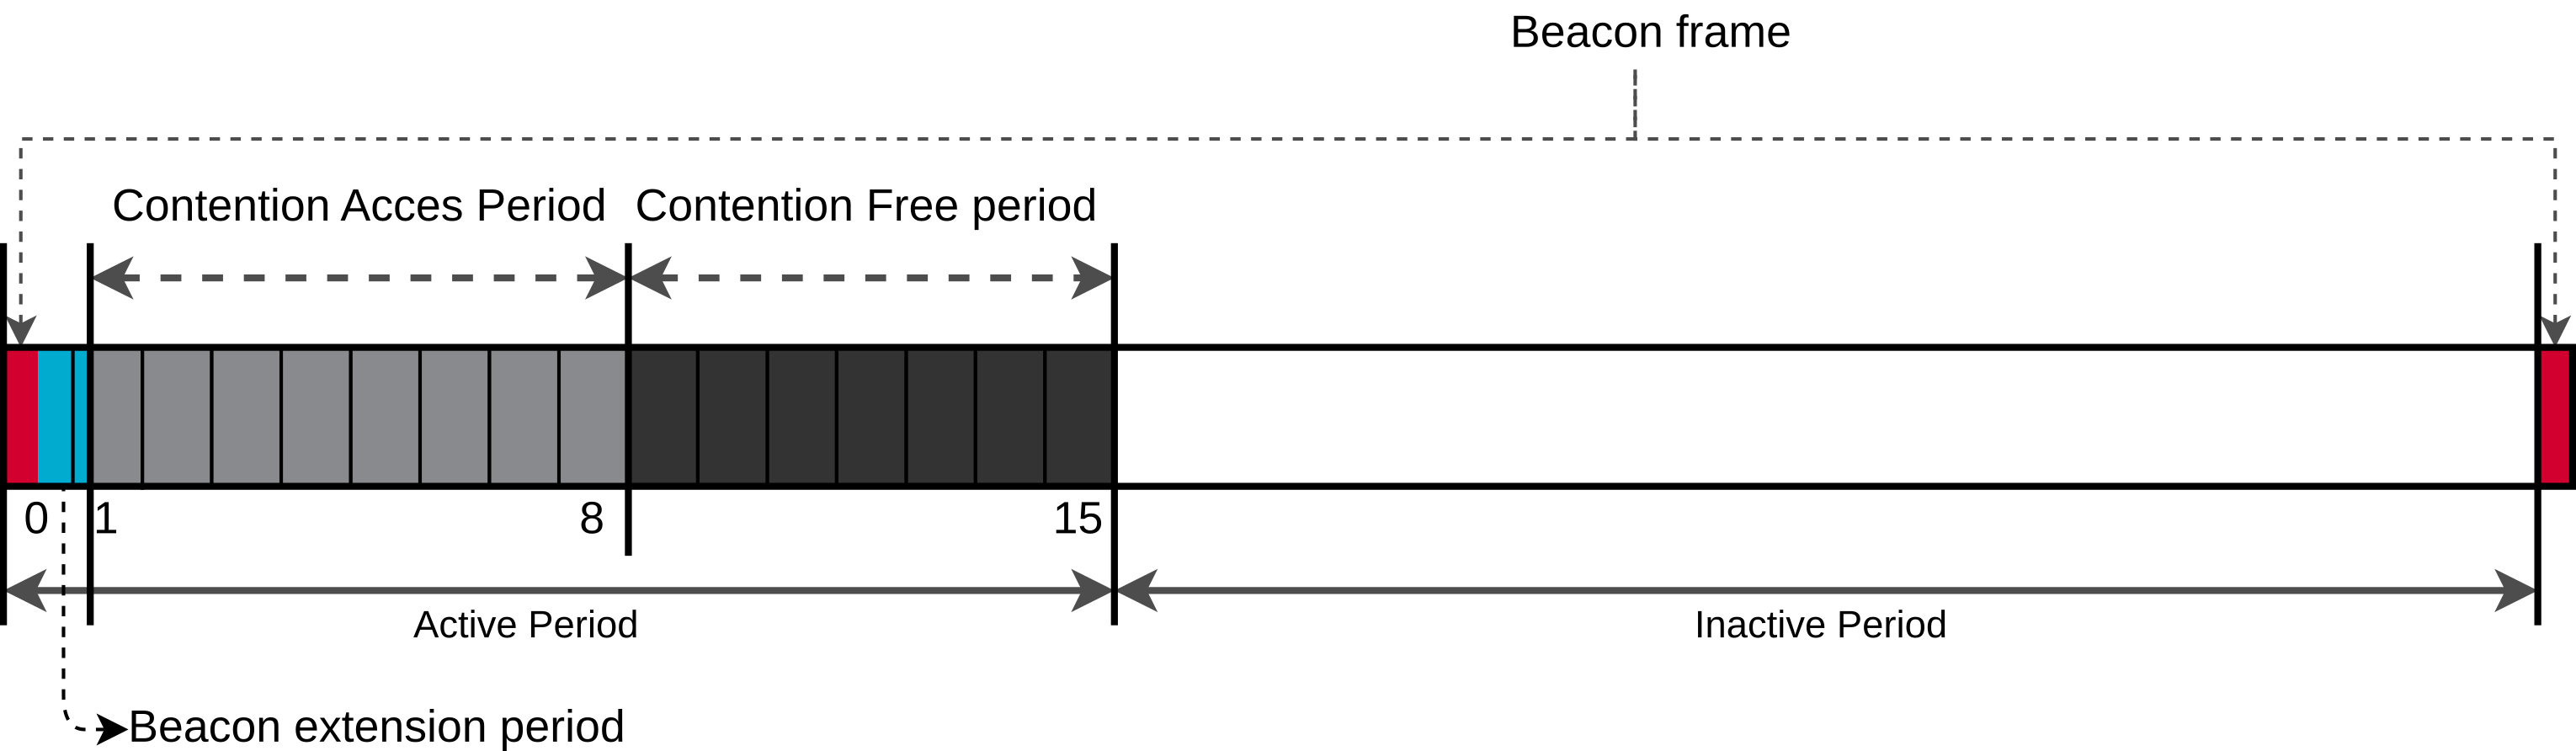
\includegraphics[scale=0.8]{res/pictures/superframe.png}
        }
        \caption{802.15.4 structure de la Superframe.}
        \label{fig:etat_art-802.15.4.superframe}
    \end{figure}

    Dans le mode Non-Beacon Enabled, il n'y a pas de synchronisation. l'accès au canal se fait par l'algorithme Unslotted CSMA-CA.


\subsection*{IEEE 802.15.4e}
    802.15.4 a un certains nombres de limitations. \cite{paper:802.15.4e-survey} met les limitations suivantes en évidence:
    \begin{itemize}
      \item Aucune garantie sur le délai maximal pour qu'un paquet puisse atteindre sa destination
        ne peut être fourni avec l'alorithme CSMA-CA.
      \item La fiabilité des communications est limitée par l'utilisation de l'algorithme slotted   CSMA-CA qui offre un taux de transmission faible.
      \item Aucune protection contre les interférences due à l'utilisation d'un seul canal et à     l'absence de mécanismes de sauts de fréquence (frequency hopping)
    \end{itemize}
    Ces limitations ont menées à la création de 802.14.4.e en 2012 qui redifinis les protocoles MAC du  standard.
    Ainsi, 5 modes de fonctionnement de la couche MAC sont introduis:
    \begin{enumerate}
      \item Time Slotted Channel Hopping (TSCH)
        %Cible les applications tel que l'automatisation de processus. Permet des communications    %multi-sauts et multi-canaux.
      \item Deterministic and Synchronous Multi-channel Extension (DSME)
        %Réalisé pour des applications industirelles et commercialesayant des contraintes de délai et
        %fiabilité. Permet des communications multi-sauts ainsi que la création de réseaux MESH.
      \item Low Latency Deterministic Network (LLDN)
        %Conçu pour les applications nécessitant une latence faible et les réseaux n'utilisant qu'un seul
        %canl pour des chemins d'un saut maximum.
      \item Asynchronous multi-channel adaptation (AMCA)
        %Cible les applications où de grands déploiments sont nécessaire comme le monitoring    %d'infrastructures.
      \item Radio Frequency Identification Blink (BLINK)
        %Conçu pour i'identification de personnes ou d'objets. Il permet aux noeuds de communiquer leur
        %ID aux autres noeuds sans avoir été préalablement associés.
    \end{enumerate}
    D'après \cite{paper:802.15.4e-survey}, le standart ne définit que brièvement AMCA et BLINK.
    LLDN est destiné aux réseaux à un seul saut et utilisant un seul canal. Il n'est donc pas pertinent pour ce projet. DSME utilise le concept de multi-superframe semblable aux superframe de IEEE 802.15.4 mise à part la CFP qui divie chacun des 7 slots en plusieurs fréquences.


\subsection{TSCH (Time Slotted Channel Hopping)}\label{subsec:etat_art-802.15.4.tsch}

Ce mode de fonctionnement de la couche MAC, comme son nom l'indique, supporte à la fois les sauts en fréquence et des communications divisées en temps. Ces mécanismes réduisent efficacement les effets des interférences et les collisions ce qui améliore la fiabilité du réseau.

\subsubsection*{Slotframe}
Dans ce mode, le concept de superframe de 802.15.4 est remplacé par le concept de slotframe.
Une slotframe est un intervalle de temps qui divisé en timeslots. Chaque timeslot permet à un noeud d'envoyer une trame et d'éventuellement recevoir son acquitement (ack).
Chaque timeslot possède un identifiant appellé \textit{Absolute Slot Number} (ASN)
et un identifiant au sein de la slotframe appelé \textit{Time Slot Number} (TSN).

TSCH permet l'utilisation de timeslots partagés et dédiés. Dans les timeslots partagés plusieurs noeuds peuvent communiquer. Dans ce cas, CSMA/CA est utilisé. Pour les timeslots dédiés, seul deux noeuds peuvent communiquer. La figure~\ref{fig:state-slotframe} illustre une slotframe composée de trois timeslots.
Dans cet exemple, on considère 3 noeuds: N, T et U. Chaque timeslot permet une communication entre deux noeud.
Par exemple le timeslot ayant comme TSN 0, permet à N de transmettre vers T.

\begin{figure}[H]
  \centering
  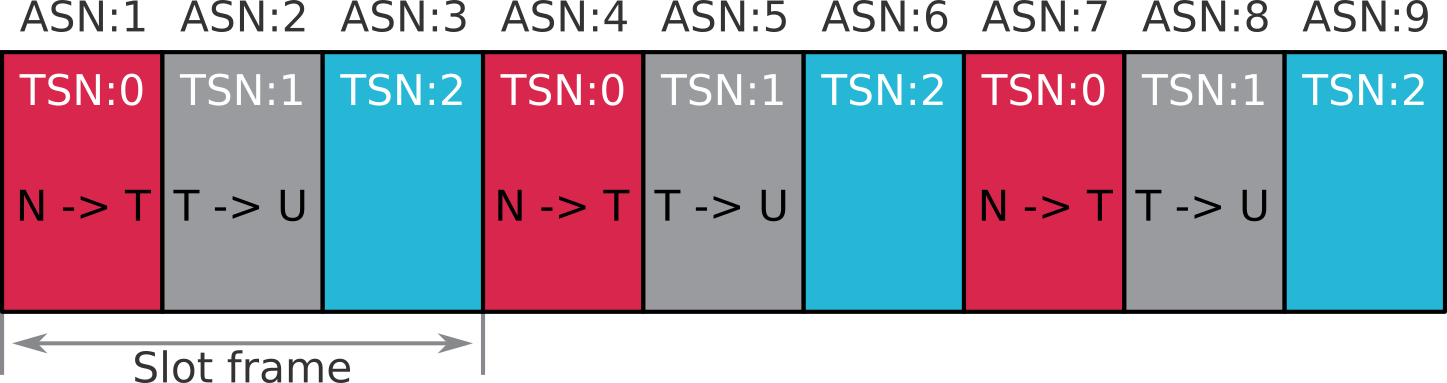
\includegraphics[scale=0.7]{res/pictures/sloframe.png}
  \caption{Slotframe.}
  \label{fig:state-slotframe}
\end{figure}

\subsubsection*{Channel Hopping}

TSCH peut utiliser 16 canaux différents numérotés de 0 à 15. Un lien entre deux noeuds dans TSCH est alors défini par la paire (timeslot, canal). Ainsi, chaque slot frame est divisiée par le nombre de canaux utilisé dans le réseau (Fig.~\ref{fig:state-tsch}). figure~\ref*{fig:state-slotframe}  Soit f la fréquence utilisée pour la communication entre deux noeuds:

\[
    f = F[(ASN + channel Offset)\% N_{channels}]
\]

où $N_{channels}$ est le nombre de canaux utilisés pour le réseau. F peut être vue comme une table qui contient une séquence de canaux.

\begin{figure}[H]
    \centering
    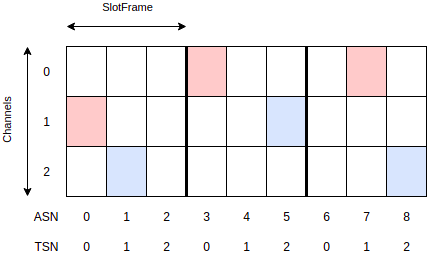
\includegraphics[scale=0.5]{res/pictures/tsch.drawio.png}
    \caption{Time Slotted Channel Hopping.}
    \label{fig:state-tsch}
\end{figure}


%\subsubsection*{Formation du PAN}

%\subsubsection*{Synchronisation en temps}
%%%%%%%%%%%%%%%%%%%%% glossaries %%%%%%%%%%%%%%%%%%%%%
%\printglossaries

%%%%%%%%%%%%%%%%%%%%% bibliography %%%%%%%%%%%%%%%%%%%%%
\bibliography{res/bibliography/main,res/bibliography/rfc}
\bibliographystyle{plain}

%%%%%%%%%%%%%%%%%%%%% notes %%%%%%%%%%%%%%%%%%%%%
%<type>:<chapter_label_name>-<label>
%types:
% - chap: chapter
% - sec: section
% - subsec: sub section
% - fig: pictures
% - tb: tables
% - ft: foot notes
% - eq: equation
%
% chapters:
% - intro
% - state
%
%%%%%%%%%%%%%%%%%%%%% structure %%%%%%%%%%%%%%%%%%%%%
% TODO
%
\end{document}
